% -*- latex -*-
%%%%%%%%%%%%%%%%%%%%%%%%%%%%%%%%%%%%%%%%%%%%%%%%%%%%%%%%%%%%%%%%
%%%%%%%%%%%%%%%%%%%%%%%%%%%%%%%%%%%%%%%%%%%%%%%%%%%%%%%%%%%%%%%%
%%%%
%%%% This text file is part of the source of 
%%%% `Parallel Programming in MPI and OpenMP'
%%%% by Victor Eijkhout, copyright 2012-8
%%%%
%%%% omp-basics.tex : intro stuff
%%%%
%%%%%%%%%%%%%%%%%%%%%%%%%%%%%%%%%%%%%%%%%%%%%%%%%%%%%%%%%%%%%%%%
%%%%%%%%%%%%%%%%%%%%%%%%%%%%%%%%%%%%%%%%%%%%%%%%%%%%%%%%%%%%%%%%

This chapter explains the basic concepts of OpenMP, and helps you get
started on running your first OpenMP program.

\Level 0 {The OpenMP model}

We start by establishing a mental picture of the hardware and software
that OpenMP targets.

\Level 1 {Target hardware}

Modern computers have a multi-layered design. Maybe you have access to
a cluster, and maybe you have learned how to use MPI to communicate
between cluster nodes. OpenMP, the topic of this chapter, is concerned
with a single \indextermsub{cluster}{node} or \indexterm{motherboard},
and getting the most out of the available parallelism available there.

\begin{figure}[ht]
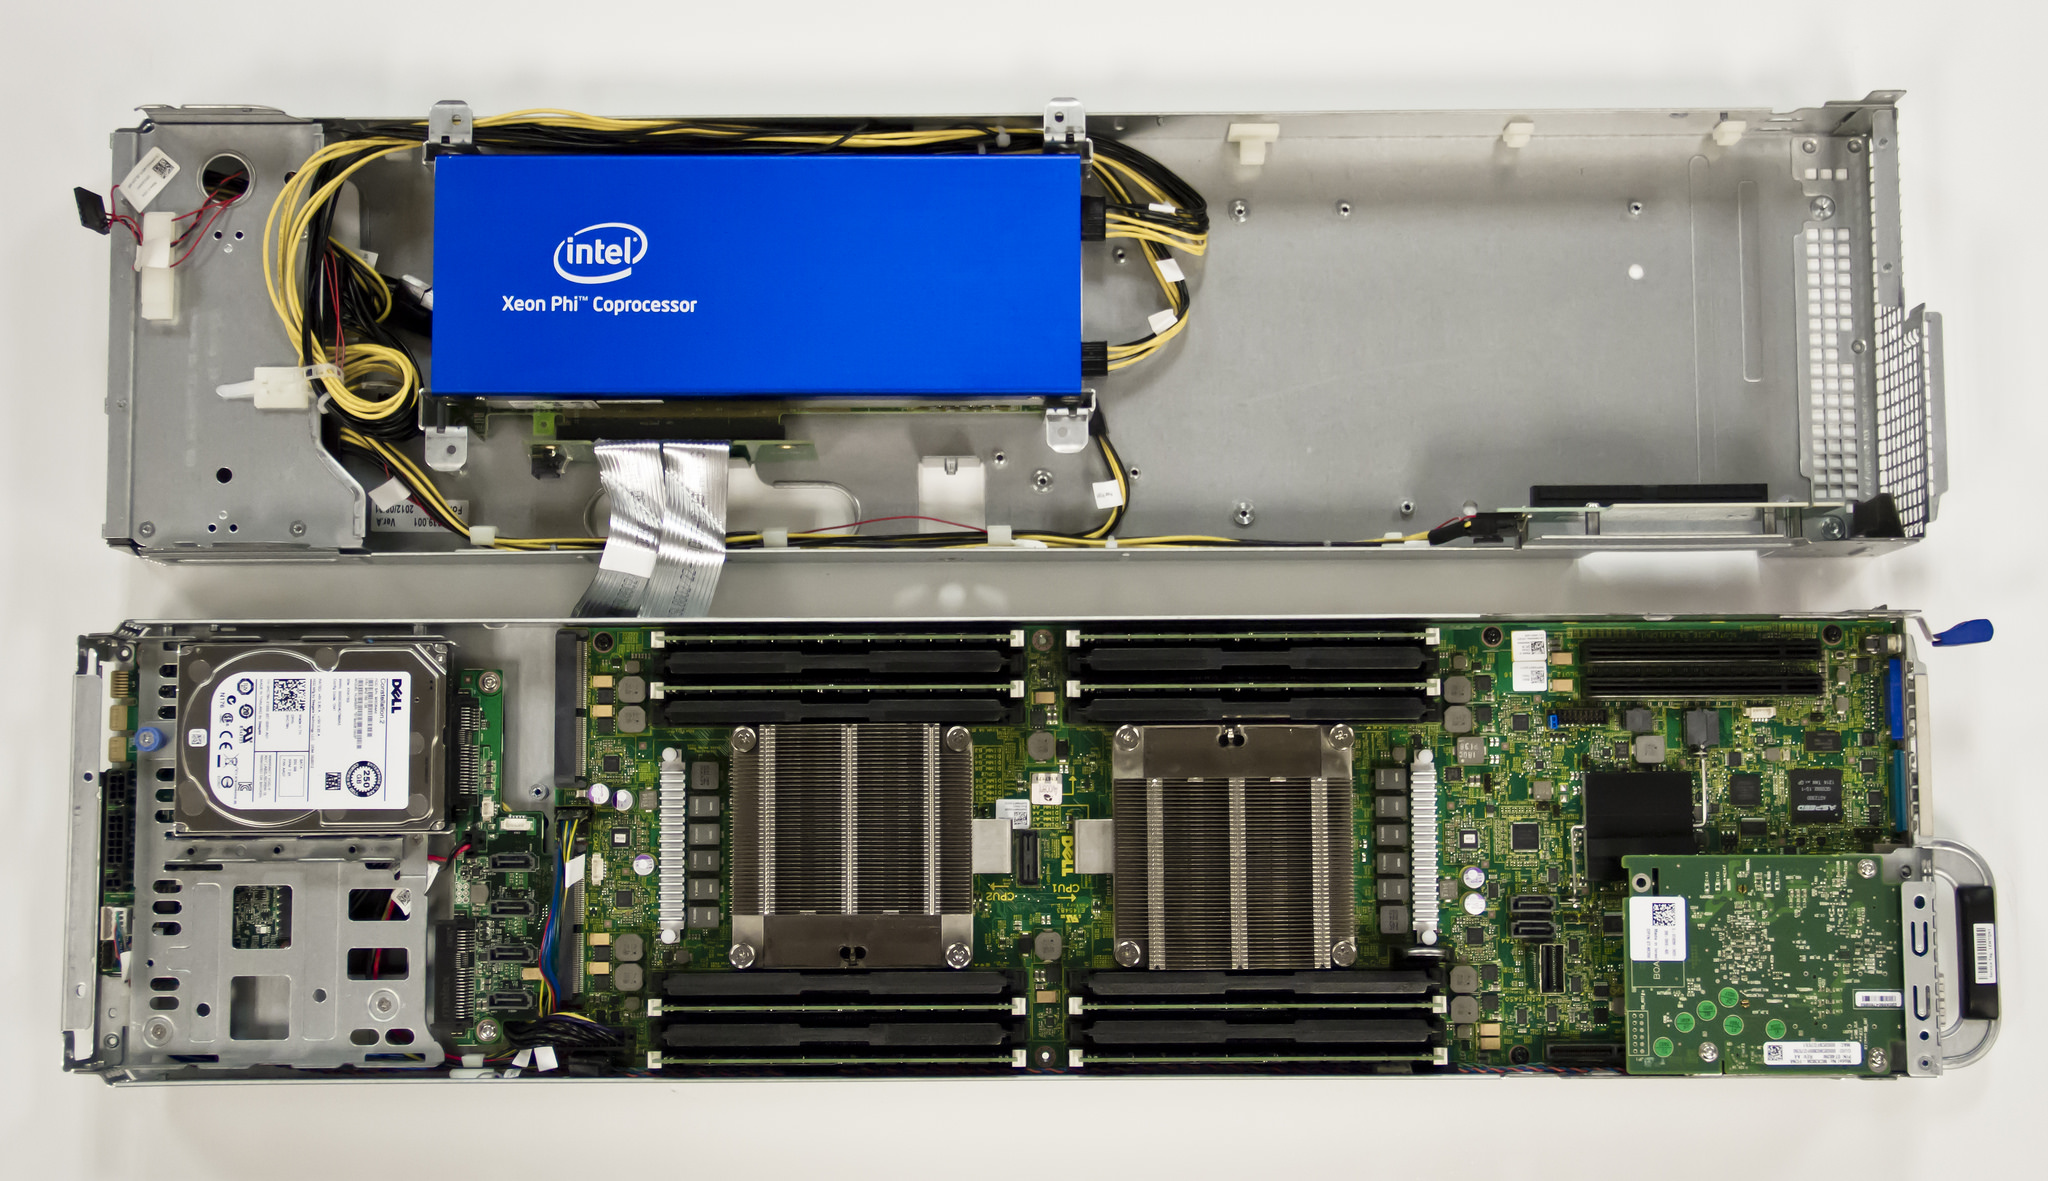
\includegraphics[scale=.13]{stampede-node}
\caption{A node with two sockets and a co-processor}
\label{fig:stampedenode}
\end{figure}
%
Figure~\ref{fig:stampedenode} pictures a typical design of a node:
within one enclosure you find two \emph{sockets}\index{socket|textbf}:
single processor chips. Your personal laptop of computer will probably
have one socket, most supercomputers have nodes with two or four
sockets (the picture is of a \indextermbus{Stampede}{node} with two
sockets)\footnote {In that picture you also see a co-processor: OpenMP
  is increasingly targeting those too.}, although the recent
\indextermbus{Intel}{Knight's Landing} is again a single-socket
design.

\begin{figure}[ht]
  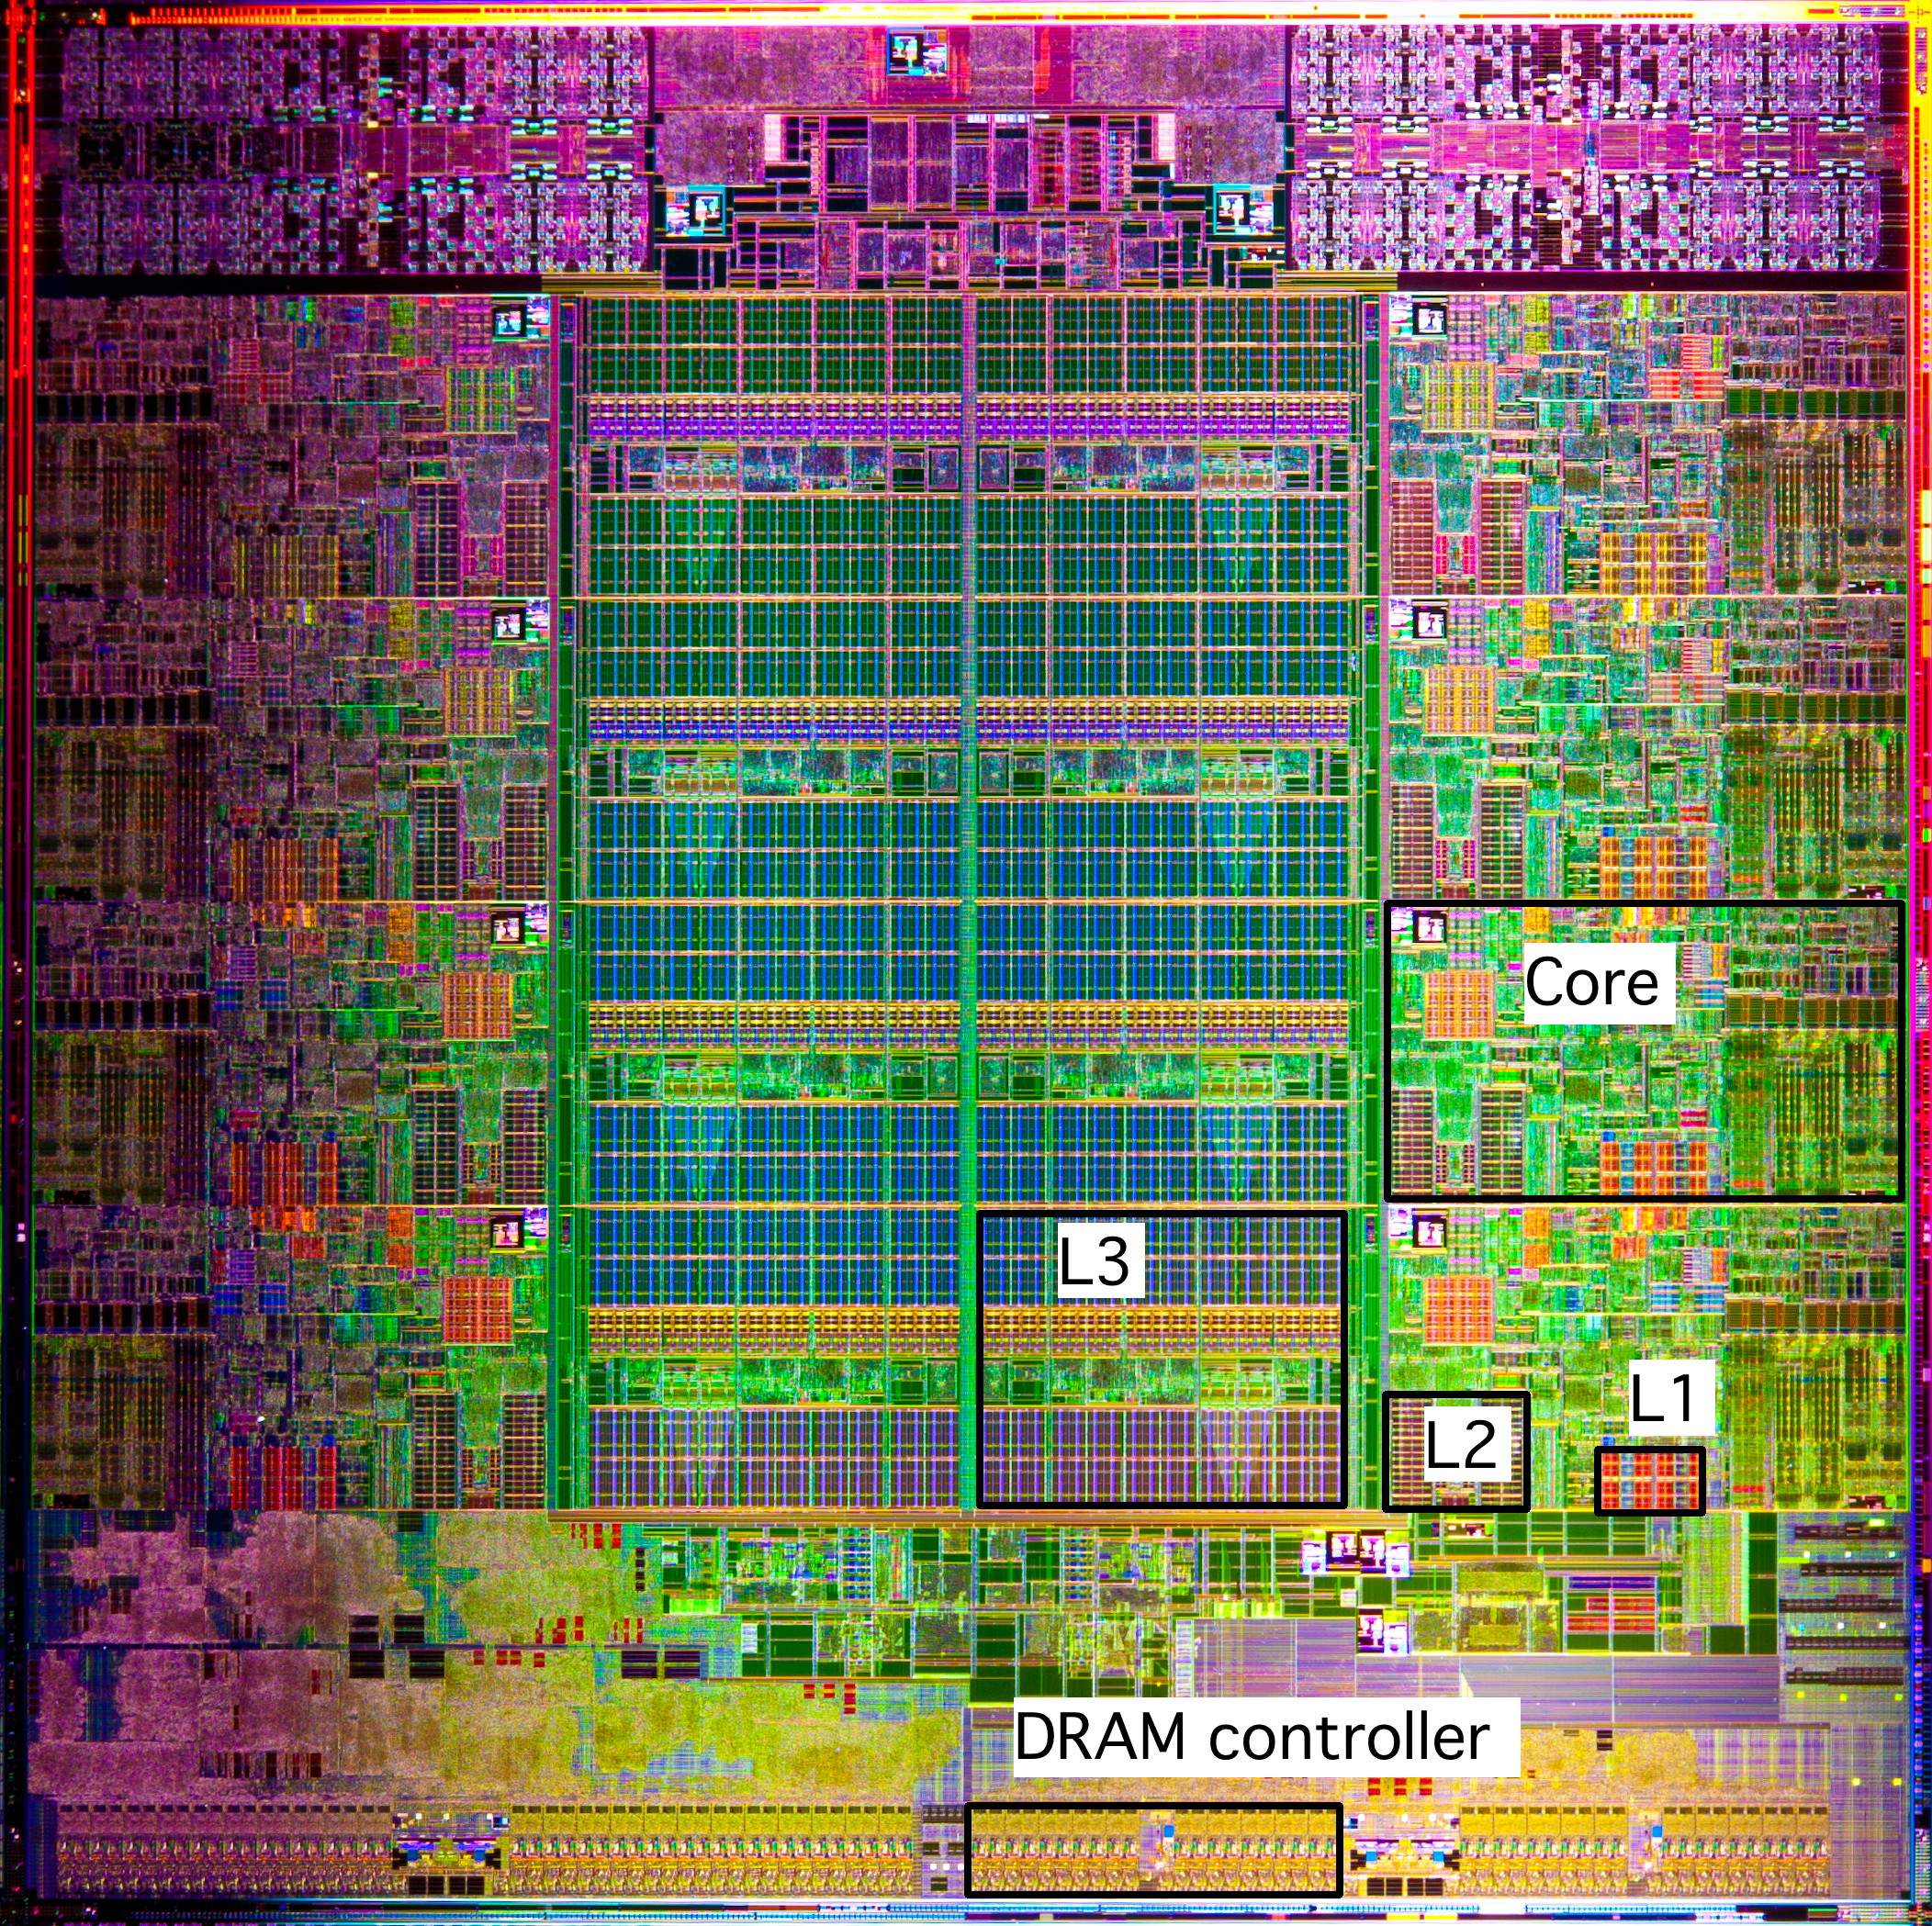
\includegraphics[scale=.45]{sandybridge-eightcore-ann}
  \caption{Structure of an Intel Sandybridge eight-core socket}
  \label{fig:sandybridge}
\end{figure}
%
To see where OpenMP operates we need to dig into the
sockets. Figure~\ref{fig:sandybridge} shows a picture of an
\indextermbus{Intel}{Sandybridge} socket. You recognize a structure
with eight \emph{cores}\indextermdef{core}: independent processing
units, that all have access to the same memory. (In
figure~\ref{fig:stampedenode} you saw four memory banks attached to
each of the two sockets; all of the sixteen cores have access to all
that memory.)

To summarize the structure of the architecture that OpenMP targets:
\begin{itemize}
\item A node has up to four sockets;
\item each socket has up to~60 cores;
\item each core is an independent processing unit, with access to all
  the memory on the node.
\end{itemize}

\Level 1 {Target software}

OpenMP is based on on two concepts: the use of \indexterm{threads}
and the \indextermdef{fork/join model} of
parallelism. For now you can think of a thread as a sort of process:
the computer executes a sequence of instructions.
The fork/join model says that a thread can split itself (`fork')
into a number of threads that are identical copies. At some point
these copies go away and the original thread is left (`join'),
but while the \indextermsub{team of}{threads} created by the fork exists,
you have parallelism available to you. The part of the execution
between fork and join is known as a \indexterm{parallel region}.

Figure~\ref{fig:forkjoin} gives a simple picture of this:
a thread forks into a team of threads, and these threads
themselves can fork again.
\begin{figure}[ht]
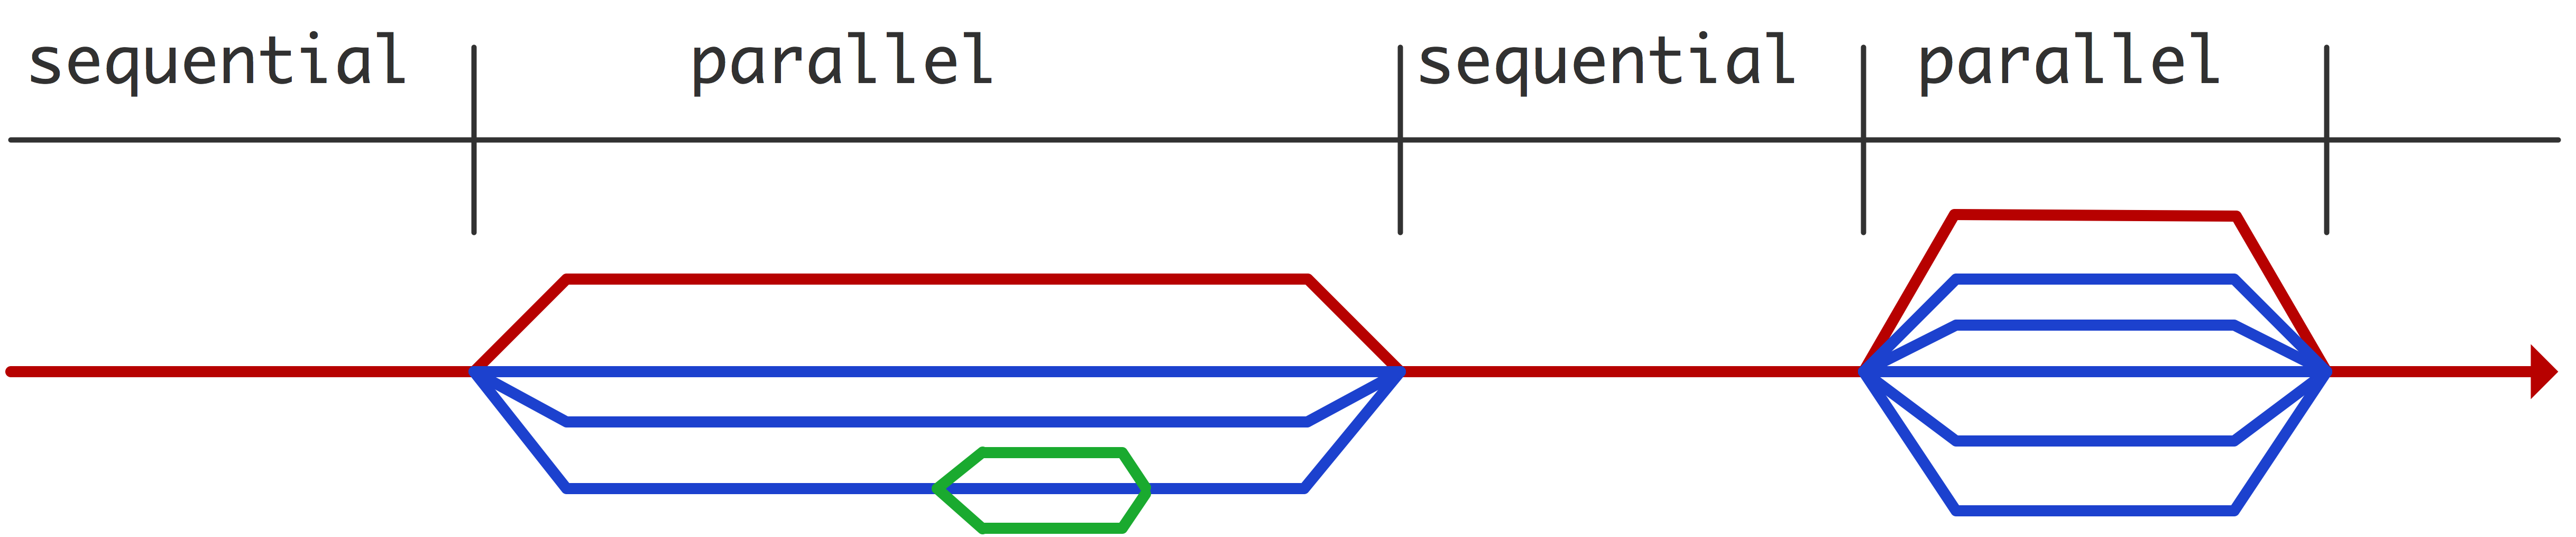
\includegraphics[scale=.08]{fork-join}
\caption{Thread creation and deletion during parallel execution}
\label{fig:forkjoin}
\end{figure}

The threads that are forked are all copies of the
\emph{master thread}\index{threads!master}: they have access to all that was
computed so far; this is their \indexterm{shared data}.  Of course, if
the threads were completely identical the parallelism would be
pointless, so they also have private data, and they can identify
themselves: they know their thread number.  This allows you to do
meaningful parallel computations with threads.

This brings us to the third important concept: that of \indexterm{work sharing}
constructs. In a team of threads, initially there will be replicated execution;
a work sharing construct divides available parallelism over the threads.

\begin{quote}
  So there you have it: OpenMP uses teams of threads, and inside
  a parallel region the work is distributed over the threads with a work sharing construct.
  Threads can access shared data, and they have some private data.
\end{quote}

An important difference between OpenMP and MPI is that parallelism in
OpenMP is dynamically activated by a thread spawning a team of
threads. Furthermore,
the number of threads used can differ between parallel regions, and
threads can create threads recursively. This is known as
as \indexterm{dynamic mode}. By contrast, in an MPI program the number
of running processes is (mostly) constant throughout the run, and
determined by factors external to the program.

\Level 1 {About threads and cores}

OpenMP programming is typically done to take advantage of
\indexterm{multicore} processors. Thus, to get a good speedup you
would typically let your number of threads be equal to the number of
cores. However, there is nothing to prevent you from creating more
threads: the operating system will use \indexterm{time slicing} to let
them all be executed. You just don't get a speedup beyond the number
of actually available cores.

On some modern processors there are \indextermsub{hardware}{threads},
meaning that a core can actually let more than thread be executed,
with some speedup over the single thread. To use such a processor
efficiently you would let the number of OpenMP threads be $2\times$ or
$4\times$ the number of cores, depending on the hardware.

\Level 1 {About thread data}

In most programming languages, visibility of data
is governed by rules on the \indextermbus{scope}{of variables}:
a~variable is declared in a block, and it is then visible to any
statement in that block and blocks with a \indextermsub{lexical}{scope}
contained in it, but not in surrounding blocks:
\begin{verbatim}
main () {
  // no variable `x' define here
  {
    int x = 5;
    if (somecondition) { x = 6; }
    printf("x=%e\n",x); // prints 5 or 6
  }
  printf("x=%e\n",x); // syntax error: `x' undefined
}
\end{verbatim}

In C, you can redeclare a variable inside a nested scope:
\begin{verbatim}
{
  int x;
  if (something) {
    double x; // same name, different entity
  }
  x = ... // this refers to the integer again
}
\end{verbatim}
Doing so makes the outer variable inaccessible.

Fortran has simpler rules, since it does not have blocks inside blocks.

\begin{figure}[ht]
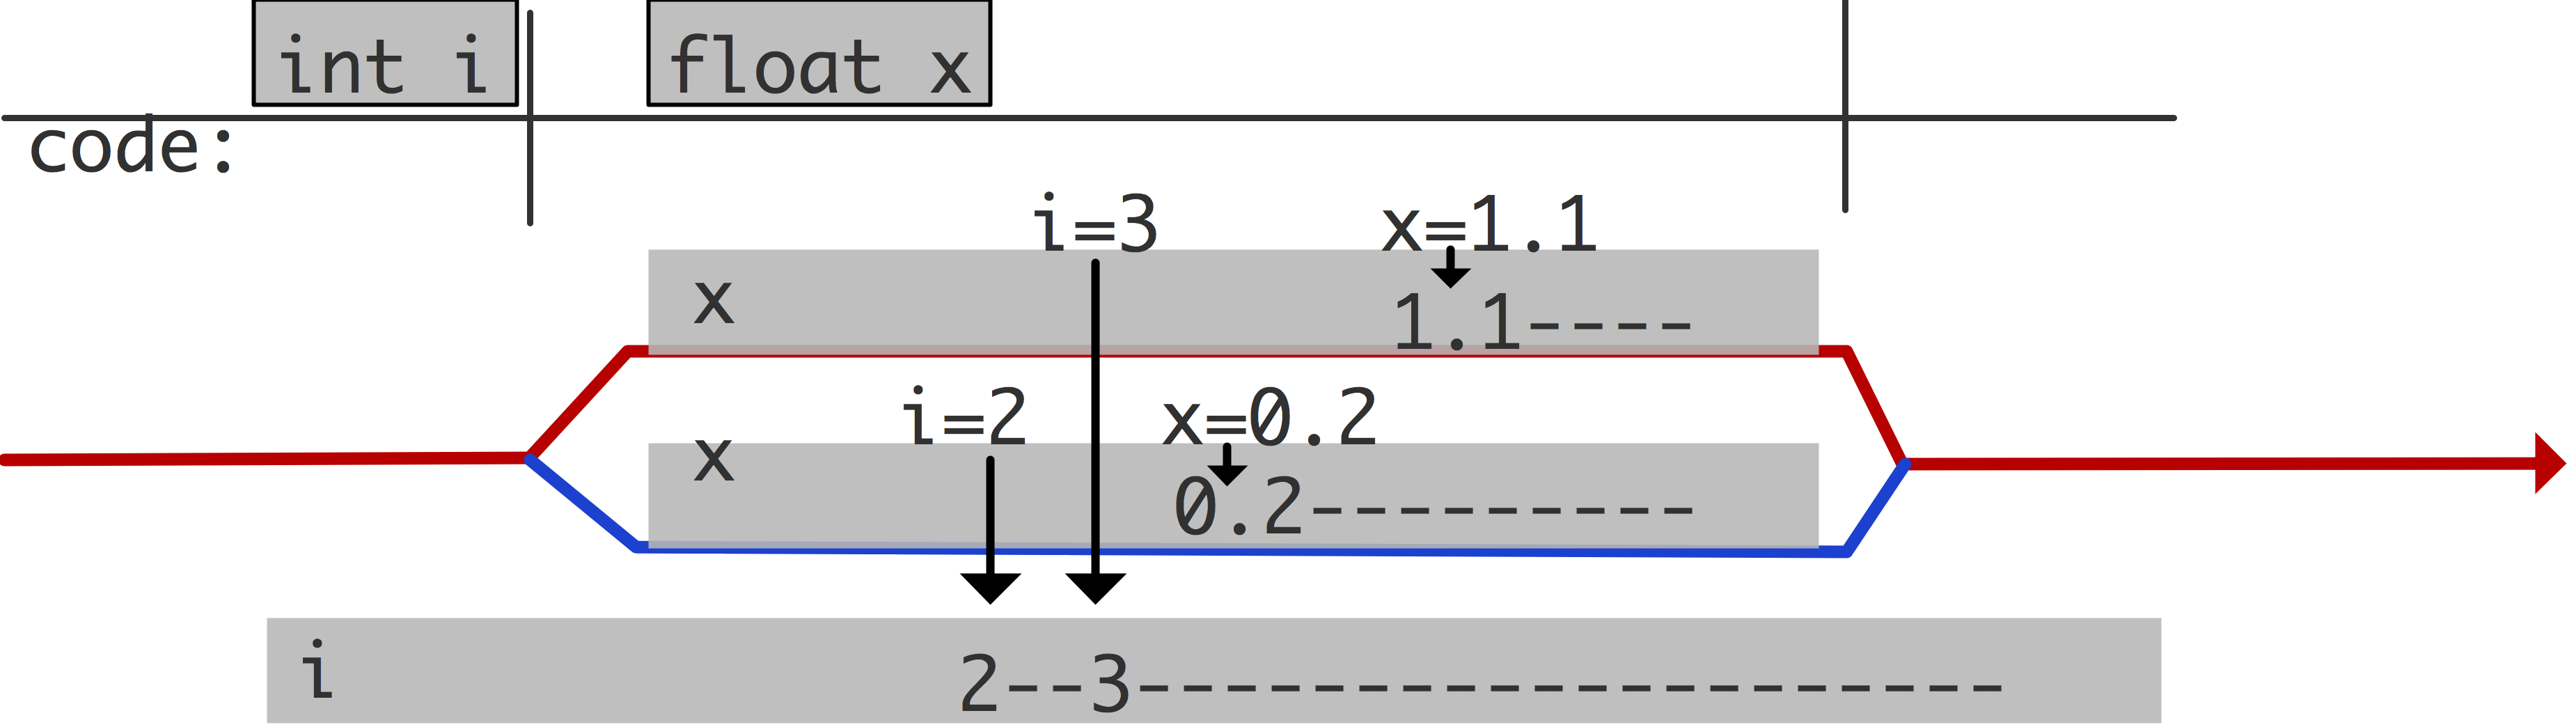
\includegraphics[scale=.1]{fork-join-vars}
\caption{Locality of variables in threads}
\label{fig:threadvars}
\end{figure}
%
In OpenMP the situation is a bit more tricky because of the threads.
When a team of threads is created they can all see the data of the
master thread. However, they can also create data of their own.
This is illustrated in figure~\ref{fig:threadvars}.
We will go into the details later.

\Level 0 {Compiling and running an OpenMP program}

\Level 1 {Compiling}
\index{OpenMP!compiling|(}

Your file or Fortran module needs to contain
\begin{verbatim}
#include "omp.h"
\end{verbatim}
in C, and 
\begin{verbatim}
use omp_lib
\end{verbatim}
or
\begin{verbatim}
#include "omp_lib.h"
\end{verbatim}
for Fortran.

OpenMP is handled by extensions to your regular compiler, typically by
adding an option to your commandline:
\begin{verbatim}
# gcc
gcc -o foo foo.c -fopenmp
# Intel compiler
icc -o foo foo.c -openmp
\end{verbatim}
If you have separate compile and link stages, you need that option in both.

When you use the openmp compiler option, a \indexterm{cpp} variable \indexompshow{_OPENMP}
will be defined. Thus, you can have conditional compilation by writing
\begin{verbatim}
#ifdef _OPENMP
   ...
#else
   ...
#endif
\end{verbatim}

\index{OpenMP!compiling|)}

\Level 1 {Running an OpenMP program}
\index{OpenMP!running|(}

You run an OpenMP program by invoking it the regular way (for instance \n{./a.out}),
but its behaviour is influenced by some \indextermbus{OpenMP}{environment variables}.
The most important one is \indexompshow{OMP_NUM_THREADS}:
\begin{verbatim}
export OMP_NUM_THREADS=8
\end{verbatim}
which sets the number of threads that a program will use.
See section~\ref{ref:omp-environ} for a list of all environment variables.

\index{OpenMP!running|)}

\Level 0 {Your first OpenMP program}

In this section you will see just enough of OpenMP to write a first
program and to explore its behaviour. For this we need to introduce a
couple of OpenMP language constructs. They will all be discussed in
much greater detail in later chapters.

\Level 1 {Directives}
\label{sec:omp-directives}
\index{directives|(textbf}

OpenMP is not magic, so you have to tell it when something
can be done in parallel. This is mostly done through \indexterm{directives};
additional specifications can be done through library calls.

In C/C++ the \indextermdef{pragma} mechanism is used: annotations for
the benefit of the compiler that are otherwise not part of the
language. This looks like:
\begin{verbatim}
#pragma omp somedirective clause(value,othervalue)
  parallel statement;

#pragma omp somedirective clause(value,othervalue)
 {
  parallel statement 1;
  parallel statement 2;
 }
\end{verbatim}
with
\begin{itemize}
\item the \verb+#pragma omp+ \indextermdef{sentinel} to indicate that
  an OpenMP directive is coming;
\item a directive, such as \n{parallel};
\item and possibly clauses with values.
\item After the directive comes either a single statement or a block
  in \indexterm{curly braces}.
\end{itemize}
Directives in C/C++ are case-sensitive. Directives can be broken over
multiple lines by escaping the line end.

The sentinel in Fortran looks like a comment:
\begin{verbatim}
!$omp directive clause(value)
  statements
!$omp end directive
\end{verbatim}
The difference with the C~directive is that
Fortran can not have a block, so there is an explicit
\indextermsub{end-of}{directive} line.

If you break a directive over more than one line, all but the last line
need to have a continuation character, and each line needs to have the sentinel:
\begin{verbatim}
!$OMP parallel do &
!%OMP   copyin(x),copyout(y)
\end{verbatim}
The directives are case-insensitive. In
\indextermbus{Fortran}{fixed-form source} files, \verb+c$omp+ and
\verb+*$omp+ are allowed too.

\index{directives|)}

\Level 1 {Parallel regions}

The simplest way to create parallelism in OpenMP is to use
the \indexpragma{parallel} pragma. A~block preceded by the \n{omp parallel} pragma
is called a \emph{parallel region}; it
is executed by a newly created team of threads. 
This is an instance of the \indexac{SPMD} model: all threads execute the same
segment of code.
\begin{verbatim}
#pragma omp parallel
{
  // this is executed by a team of threads
}
\end{verbatim}

We will go into much more detail in section~\ref{sec:parallelregion}.

\Level 1 {An actual OpenMP program!}

\begin{exercise}
  \label{ex:omp-procthread}
  Write a program that contains the following lines:
\begin{verbatim}
  printf("There are %d processors\n",omp_get_num_procs());
#pragma omp parallel
  printf("There are %d threads\n",
        /* !!!! something missing here !!!! */ );
\end{verbatim}
The first print statement tells you the number of available cores in
the hardware. Your assignment is to
supply the missing function that reports the number
of threads used. Compile and run the program. Experiment with the
\n{OMP_NUM_THREADS} environment variable. What do you notice about the
number of lines printed?
\end{exercise}

\begin{exercise}
  \label{ex:omp-procthreadn}
  Extend the program from exercise~\ref{ex:omp-procthread}. Make a
  complete program based on these lines:
\begin{verbatim}
int tsum=0;
#pragma omp parallel
  tsum += /* the thread number */
printf("Sum is %d\n",tsum);
\end{verbatim}
Compile and run again. (In fact, run your program a number of times.)
Do you see something unexpected? Can you think
of an explanation?
\end{exercise}

\Level 1 {Code and execution structure}
\label{sec:omp-code-structure}

Here are a couple of important concepts:
\begin{definition}
\item[structured block] An OpenMP directive is followed by an
  \indexterm{structured block}; in C~this is a single statement, a
  compound statement, or a block in braces; In Fortran it is
  delimited by the directive and its matching `\n{end}' directive.

  A~structured block can not be jumped into, so it can not start with a
  labeled statement, or contain a jump statement leaving the block.
\item[construct] An OpenMP \indexterm{construct} is the section of code
  starting with a directive and spanning the following structured block,
  plus in Fortran the end-directive. This is a lexical concept: it contains
  the statements directly enclosed, and not any subroutines called from them.
\item[region of code] A \indexterm{region of code} is defined as all statements
  that are dynamically encountered while executing the code of an OpenMP construct.
  This is a dynamic concept: unlike a `construct', it does include any subroutines
  that are called from the code in the structured block.
\end{definition}

\endinput

\Level 0 {Thread data}

In most programming languages, visibility of data
is governed by rules on the \indextermbus{scope}{of variables}:
a~variable is declared in a block, and it is then visible to any
statement in that block and blocks with a \indextermsub{lexical}{scope}
contained in it, but not in surrounding blocks:
\begin{verbatim}
main () {
  // no variable `x' define here
  {
    int x = 5;
    if (somecondition) { x = 6; }
    printf("x=%e\n",x); // prints 5 or 6
  }
  printf("x=%e\n",x); // syntax error: `x' undefined
}
\end{verbatim}
Fortran has simpler rules, since it does not have blocks inside blocks.

OpenMP has similar rules concerning data in parallel regions
and other OpenMP constructs. First of all, data is visible
in enclosed scopes:
\begin{verbatim}
main() {
  int x;
#pragma omp parallel
  {
     // you can use and set `x' here
  }
  printf("x=%e\n",x); // value depends on what
                      // happened in the parallel region
}
\end{verbatim}

In C, you can redeclare a variable inside a nested scope:
\begin{verbatim}
{
  int x;
  if (something) {
    double x; // same name, different entity
  }
  x = ... // this refers to the integer again
}
\end{verbatim}
Doing so makes the outer variable inaccessible.

OpenMP has a similar mechanism:
\begin{verbatim}
{
  int x;
#pragma omp parallel
  {
    double x;
  }
}
\end{verbatim}
There is an important difference: each thread in the team
gets its own instance of the enclosed variable.

\begin{figure}[ht]
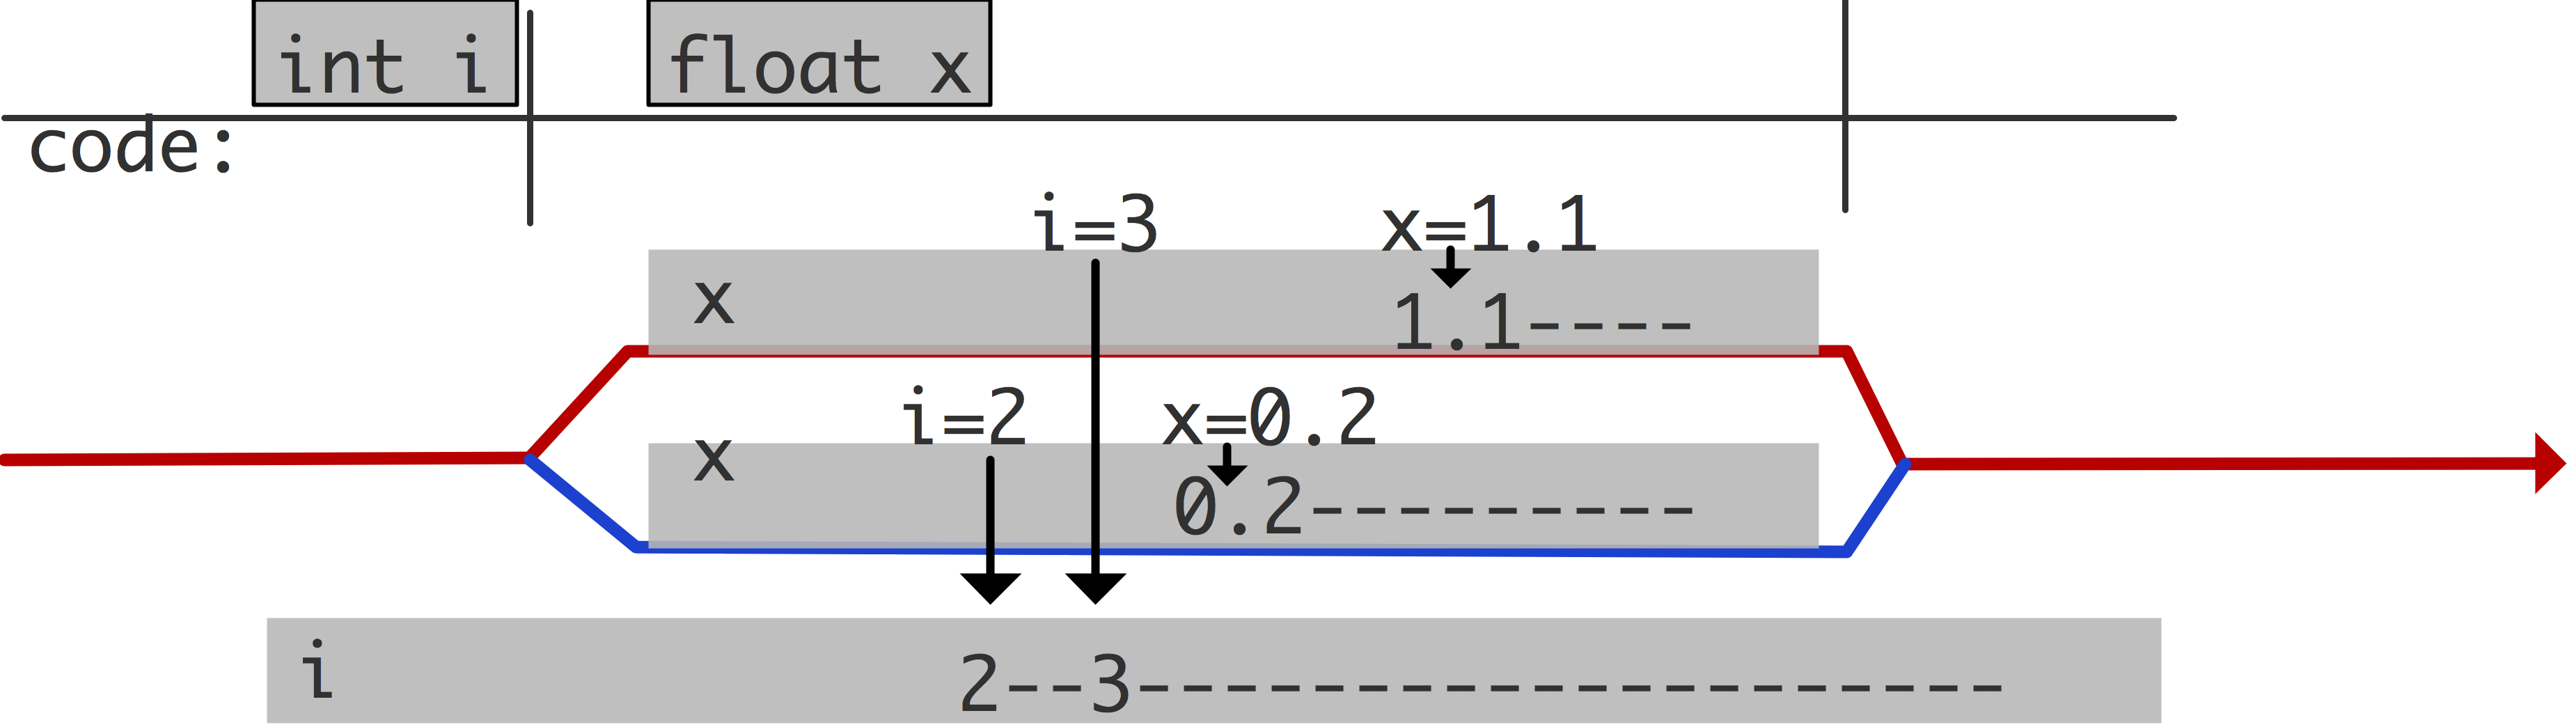
\includegraphics[scale=.1]{fork-join-vars}
\caption{Locality of variables in threads}
\label{fig:threadvars}
\end{figure}
%
This is illustrated in figure~\ref{fig:threadvars}.

In addition to such scoped variables, which live on a \indexterm{stack},
there are variables on the
\indexterm{heap}, typically created by a call to \indextermtt{malloc}
(in~C) or \indextermtt{new} (in~C++). Rules for them are more complicated.

Summarizing the above, there are
\begin{itemize}
\item \indexterm{shared variables},
  where each thread refers to the same data item, and 
\item \indexterm{private variables},
  where each thread has its own instance.
\end{itemize}
In addition to using scoping, OpenMP also uses options on the directives
to control whether data is private or shared.

Many of the difficulties of parallel programming with OpenMP stem
from the use of shared variables. For instance, if two threads
update a shared variable, you not guarantee an order on the updates.

We will discuss all this in detail in section~\ref{sec:ompdata}.

\Level 0 {Creating parallelism}
\label{sec:omp-howmany}

The \indexterm{fork/join model} of OpenMP means that you need some way of
indicating where an activity can be forked for independent execution.
There are two ways of doing this:
\begin{enumerate}
\item You can declare a parallel region and
  split one thread into a whole team of threads. We will discuss this next
  in section~\ref{sec:parallelregion}. The division of the work over the threads
  is controlled by \indexterm{work sharing construct} (section~\ref{sec:work-sharing}).
\item Alternatively, you can use tasks and indicating one parallel
  activity at a time. You will see this in section~\ref{sec:omp:task}.
\end{enumerate}

Note that OpenMP only indicates how much parallelism is present;
whether independent activities are in fact executed in parallel
is a runtime decision. The factors influencing this are discussed
in section~\ref{sec:omp-howmany}.

Declaring a parallel region tells OpenMP that a team of threads can be created.
The actual size of the team depends on various factors (see section~\ref{ref:omp-environ}
for variables and functions mentioned in this section).
\begin{itemize}
\item The \emph{environment variable}\index{OpenMP!environment variables}
  \indexompshow{OMP_NUM_THREADS} limits the number of
  threads that can be created.
\item If you don't set this variable, you can also set this limit
  dynamically with the \emph{library routine}\index{OpenMP!library
    routines} \indexompshow{omp_set_num_threads}. This routine takes
  precedence over the aforementioned environment variable if both are
  specified.
\item A limit on the number of threads can also be set as a clause
  on a parallel region.
\end{itemize}
If you specify a greater amount of parallelism than the hardware supports,
the runtime system will probably ignore your specification and choose a lower value.
To ask how much parallelism is actually used in your parallel region,
use \indexompshow{omp_get_num_threads}. To query these hardware limits,
use \indexompshow{omp_get_num_procs}.

Another limit on the number of threads is imposed when you use nested parallel regions.
This can arise if you have a parallel region in a subprogram which is sometimes called
sequentially, sometimes in parallel. The variable \indexompshow{OMP_NESTED} controls
whether the inner region will create a team of more than one thread.

